%%% LaTeX Template: Article/Thesis/etc. with colored headings and special fonts
%%%
%%% Source: http://www.howtotex.com/
%%% Feel free to distribute this template, but please keep to referal to http://www.howtotex.com/ here.
%%% February 2011
%%%
%%% Modified January 2016 by CDM

%%%  Preamble
\documentclass[11pt,letterpaper]{article}
\usepackage[margin=1.0in]{geometry}
\usepackage[T1]{fontenc}
\usepackage[bitstream-charter]{mathdesign}
\usepackage[latin1]{inputenc}					
\usepackage{amsmath}						
\usepackage{xcolor}
\usepackage{cite}
\usepackage{hyphenat}
\usepackage{graphicx}
\usepackage{float}
\usepackage{subfigure}
\usepackage{sectsty}
\usepackage[compact]{titlesec} 
\usepackage[tablegrid]{vhistory}
\usepackage{pbox}
\allsectionsfont{\color{accentcolor}\scshape\selectfont}

%%% Definitions
\definecolor{accentcolor}{rgb}{0.0,0.0,0.5} 
\newcommand{\teamname}{The Under Achievers}
\newcommand{\productname}{Synthify}
\newcommand{\coursename}{CSE 4316: Senior Design I}
\newcommand{\semester}{Fall 2018}
\newcommand{\docname}{Architectural Design Specification}
\newcommand{\department}{Department of Computer Science \& Engineering}
\newcommand{\university}{The University of Texas at Arlington}
\newcommand{\authors}{Dominic Young \\ Endy Pluviose \\ Kolten Sturgill \\ Mary Huerta \\ Mitchel Smith \\ Minh-Quan Nguyen}

%%% Headers and footers
\usepackage{fancyhdr}
	\pagestyle{fancy}						% Enabling the custom headers/footers
\usepackage{lastpage}	
	% Header (empty)
	\lhead{}
	\chead{}
	\rhead{}
	% Footer
	\lfoot{\footnotesize \teamname \ - \semester}
	\cfoot{}
	\rfoot{\footnotesize page \thepage\ of \pageref{LastPage}}	% "Page 1 of 2"
	\renewcommand{\headrulewidth}{0.0pt}
	\renewcommand{\footrulewidth}{0.4pt}

%%% Change the abstract environment
\usepackage[runin]{abstract}			% runin option for a run-in title
%\setlength\absleftindent{30pt}			% left margin
%\setlength\absrightindent{30pt}		% right margin
\abslabeldelim{\quad}	
\setlength{\abstitleskip}{-10pt}
\renewcommand{\abstractname}{}
\renewcommand{\abstracttextfont}{\color{accentcolor} \small \slshape}	% slanted text

%%% Start of the document
\begin{document}

%%% Cover sheet
{\centering \huge \color{accentcolor} \sc \textbf{\department \\ \university} \par}
\vspace{1 in}
{\centering \huge \color{accentcolor} \sc \textbf{\docname \\ \coursename \\ \semester} \par}
\vspace{0.5 in}
\begin{figure}[h!]
	\centering
   	
\includegraphics[width=0.46\textwidth]{images/underachievers.png}
\end{figure}
\vspace{0.3 in}
{\centering \huge \color{accentcolor} \sc \textbf{\teamname \\ \productname} \par}
\vspace{0.5 in}
{\centering \large \sc \textbf{\authors} \par}
\newpage


%\vspace{1 in}
%\centerline{January 13th, 2012}
%\newpage

%%% Revision History
\begin{versionhistory}
  	\vhEntry{0.1}{11.30.2018}{DY, EP, MH, KS, MS, QN}{document creation}
\end{versionhistory}
\newpage

%%% Table of contents
\setcounter{tocdepth}{2}
\tableofcontents
\newpage

%%% List of figures and tables (optional)
\listoffigures
% \listoftables
\newpage

%%% Document sections
\section{Introduction}
Synthify will get playlists from a user from each platform to bring them all together and have the playlists unified under one service. The service will auto-update after a certain amount of time has passed to make sure it's consistent with any playlist changes that the user may have done on the respective platform. The "look and feel" of Synthify is similar to Spotify's dashboard. Users should expect to listen to music from each platform they have signed up for.
\newpage
\section{System Overview}
Explain, at a high level, how you will implement a solution to the problem. Include a diagram of major components to the system (not a full architectural design, but a high level overview of the major system components and how a user or external system might interface). Avoid specific implementation details (operating system, programming languages, etc.). This section should occupy at least 1 full page.
\newpage
\section{Subsystem Definitions \& Data Flow}
This section breaks down your layer abstraction to another level of detail. Here you grapically represent the logical subsytems that compose each layer and show the interactions/interfaces between those subsystems. A subsystem can be thought of as a programming unit that implements one of the major functions of the layer. It, therefore, has data elements that serve as source/sinks for other subsystems. The logical data elements that flow between subsystems need to be explicitly defined at this point, beginning with a data flow-like diagram based on the block diagram.

\begin{figure}[h!]
	\centering
 	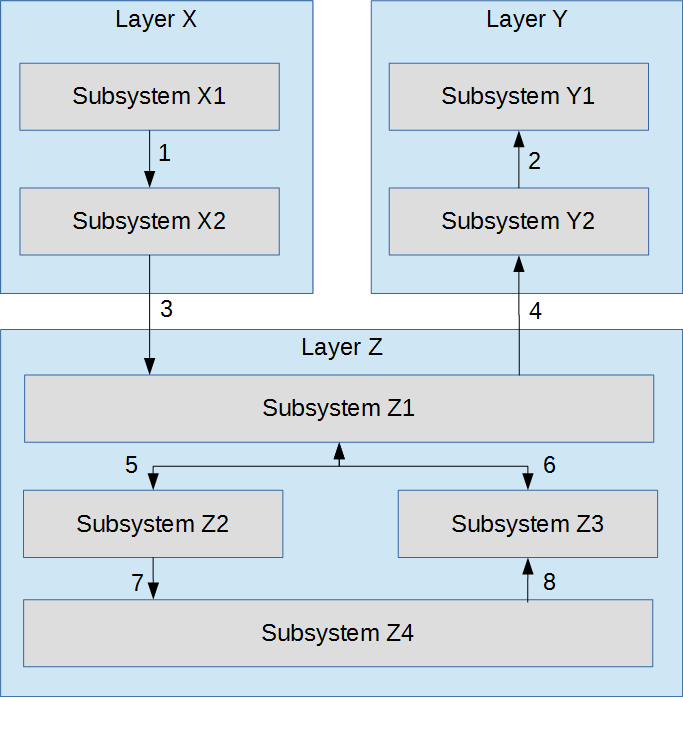
\includegraphics[width=\textwidth]{images/data_flow}
 \caption{A simple data flow diagram}
\end{figure}

\newpage
\section{Client}
The client is broken down to different components. The main component for the client will be the Redux state interface, which will keep track of states happening in the application. Other components include logging in as an existing user, registering as a new user, searching through your content once you have connected your accounts from different music platforms, the media player itself, user settings, playlists, oauth, and finally the interface, that will bring it together with the server.

\begin{figure}[h!]
	\centering
 	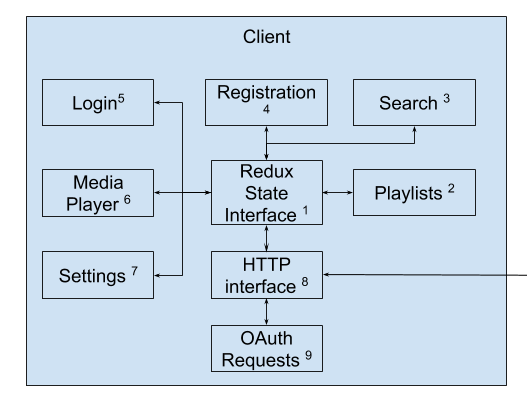
\includegraphics[width=0.60\textwidth]{images/client/ADS-SDS-Client.png}
 	\caption{Client Subsystem}
\end{figure}

\newpage

\subsection{Redux}
This subsystem allows the Client Layer to interact with the HTTP Interface. It will give information to all the different subsystems.

\begin{figure}[h!]
	\centering
 	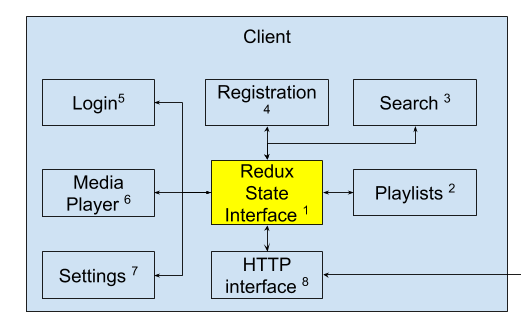
\includegraphics[width=0.60\textwidth]{images/client/client_redux.png}
 	\caption{Redux subsystem}
\end{figure}

\subsubsection{Assumptions}
We are assuming the user is using Google Chrome, and the user does not require any accessibility needs for browsing/searching.

\subsubsection{Responsibilities}
The Redux Interface responsibilities include logging in and registering users, organizing the results from the search, and creating/editing/deleting the playlists from the various third party sources (e.g. Spotify, YouTube).

\subsubsection{Subsystem Interfaces}
\begin {table}[H]
\caption {Redux interfaces} 
\begin{center}
    \begin{tabular}{ | p{1cm} | p{6cm} | p{3cm} | p{3cm} |}
    \hline
    ID & Description & Inputs & Outputs \\ \hline
    \#1 & Playlists & \pbox{3cm}{N/A} & \pbox{3cm}{List of song information from specific Playlist}  \\ \hline
    \#2 & Search & \pbox{3cm}{Search Term} & \pbox{3cm}{Playlists}  \\ \hline
    \#3 & Registration & \pbox{3cm}{E-mail \\ Password \\ Name} & \pbox{3cm}{N/A}  \\ \hline
    \#4 & Login & \pbox{3cm}{E-mail \\ Password} & \pbox{3cm}{N/A}  \\ \hline
    \#5 & Media Player & \pbox{3cm}{ Paused \\ Volume} & \pbox{3cm}{Song Functionality}  \\ \hline
    \#6 & Settings & \pbox{3cm}{N/A} & \pbox{3cm}{Output 1}  \\ \hline
    \end{tabular}
\end{center}
\end{table}

\newpage

\subsection{Playlist}
This subsystem will contain all the information on a users playlists and display it to them.

\begin{figure}[h!]
	\centering
 	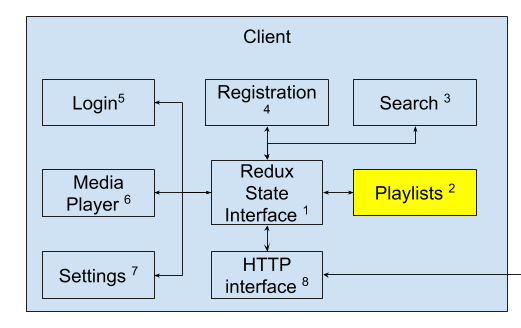
\includegraphics[width=0.60\textwidth]{images/client/client_playlists.png}
 	\caption{Playlist subsystem}
\end{figure}

\subsubsection{Subsystem Hardware}
No hardware is used for this layer. The playlist component will be a component of the home page which will be hosted on Heroku.

\subsubsection{Subsystem Operating System}
No OS is required in order for the playlist component to work properly.

\subsubsection{Subsystem Software Dependencies}
We will be using React.js 16.8.0-alpha.1 for our framework and will be using the Fetch API from Mozilla.

\subsubsection{Subsystem Programming Languages}
We will be using JavaScript ES6

\subsubsection{Subsystem Data Structures}
The data structure of the playlist is going to be an object that contains a playlist name as the key with its value being an object of song names and artists. This structure may change depending on what various music services API returns.

\subsubsection{Subsystem Data Processing}
When a use chooses a playlist that they would like to view, the Front End will take that choice in order to display the proper playlist by comparing it to the stored music data.

\newpage
\subsection{Search}
This subsection will allow users to search for playlists on their music accounts through Synthify.

\begin{figure}[h!]
	\centering
 	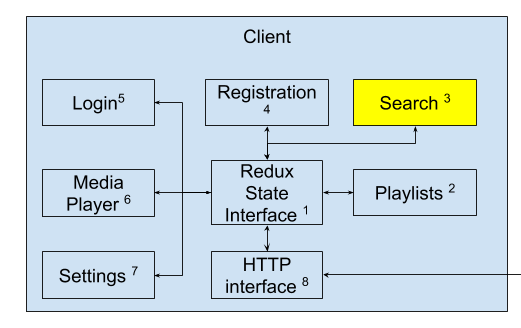
\includegraphics[width=0.60\textwidth]{images/client/client_search.png}
 	\caption{Search subsystem}
\end{figure}

\subsubsection{Subsystem Hardware}
No specific hardware will be used for searching.

\subsubsection{Subsystem Operating System}
No OS required. This will run through supported browsers such as Chrome 42 and Firefox 39.

\subsubsection{Subsystem Software Dependencies}
We will be using React.js 16.8.0-alpha, React-Router 4.3, Material-UI v3.9.0

\subsubsection{Subsystem Programming Languages}
JavaScript ES6 will be used.

\subsubsection{Subsystem Data Structures}
A fetch request will be made to the server. It will return an array of hashmaps that contains information such as artist name, song title, cover art and more.

\newpage

\subsection{Login}
This subsystem is a graphical user interface that allows a user to log into Synthify

\begin{figure}[h!]
	\centering
 	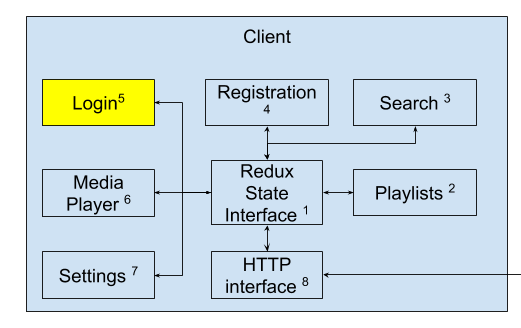
\includegraphics[width=0.60\textwidth]{images/client/client_login.png}
 	\caption{Login subsystem}
\end{figure}

\subsubsection{Assumptions}
One assumptions made is that the user will have an account in order to login.

\subsubsection{Responsibilities}
The login page will be responsible for recording the user's email and password, which will be sent to the Server subsystem via the HTTP interface.

\subsubsection{Subsystem Interfaces}
\begin {table}[H]
\caption {Login interfaces} 
\begin{center}
    \begin{tabular}{ | p{1cm} | p{6cm} | p{3cm} | p{3cm} |}
    \hline
    ID & Description & Inputs & Outputs \\ \hline
    \#01 & User found & \pbox{3cm}{User's E-mail \\ User's Password} & \pbox{3cm}{HTTP 200 OK, JSON object containing information}  \\ \hline
    \#02 & User not found or password incorrect & \pbox{4cm}{Invalid Login E-Mail \\ Incorrect Password} & \pbox{3cm}{HTTP 404, JSON Object containing error message}  \\ \hline
    \end{tabular}
\end{center}
\end{table}

\newpage

\subsection{Media Player}
This subsystem is apart of the graphical interface that allows the user to play/stop a song streaming from a third party music service.

\begin{figure}[h!]
	\centering
 	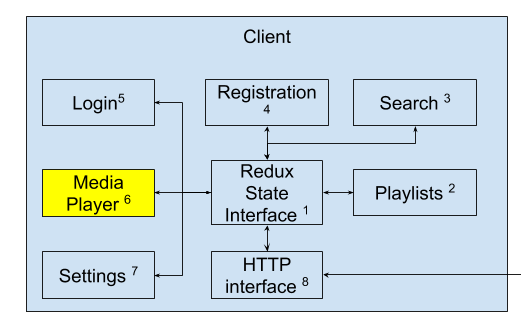
\includegraphics[width=0.60\textwidth]{images/client/client_media.png}
 	\caption{Media player subsystem}
\end{figure}

\subsubsection{Assumptions}
Assuming that the URL's that are sent from the third party music services are valid and are able to be streamed without any geographic restrictions.

\subsubsection{Responsibilities}
The Media Player subsystem is responsible for displaying the albums artwork (if available), and loading and playing/stopping a song from a remote URL from a third party music services. It also displays the remaining time left in the song.

\subsubsection{Subsystem Interfaces}
\begin {table}[H]
\caption {Media player interfaces} 
\begin{center}
    \begin{tabular}{ | p{1cm} | p{6cm} | p{3cm} | p{3cm} |}
    \hline
    ID & Description & Inputs & Outputs \\ \hline
    \#xx & Play song, HTTP request & \pbox{3cm}{Clicking Play} & \pbox{3cm}{Displays Artwork, music plays through user's speakers}  \\ \hline
    \end{tabular}
\end{center}
\end{table}

\newpage
\subsection{Settings}
The settings subsystem allows users to changed their user account information. A user can add more music accounts (SoundCloud, Spotify, etc), logout, and change the theme.

\begin{figure}[h!]
	\centering
 	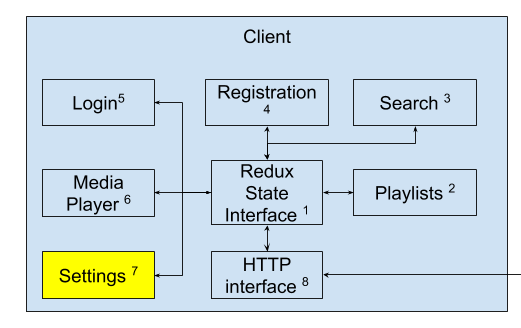
\includegraphics[width=0.60\textwidth]{images/client/client_settings.png}
 	\caption{Settings subsystem}
\end{figure}

\subsubsection{Assumptions}
One assumption made is that the user will be logged in before accessing the settings.

\subsubsection{Responsibilities}
This subsystem's primary responsibility is to allow a user to change their user information. The settings subsystem will be able to interact the with the Redux State interface to change the users theme, log them out, and add a music account to their Synthify account.

\subsubsection{Subsystem Interfaces}
\begin {table}[H]
\caption {Settings interfaces} 
\begin{center}
    \begin{tabular}{ | p{1cm} | p{6cm} | p{3cm} | p{3cm} |}
    \hline
    ID & Description & Inputs & Outputs \\ \hline
    \#01 & Redux State Interface & \pbox{3cm}{Account setting to be changed \\ user} & \pbox{3cm}{Changed setting}  \\ \hline
    \end{tabular}
\end{center}
\end{table}

\newpage

\subsection{HTTP Interface}
This interface will be the library used for the server that will direct the incoming request to the controllers via a HTTP/TCP socket.

\begin{figure}[h!]
	\centering
 	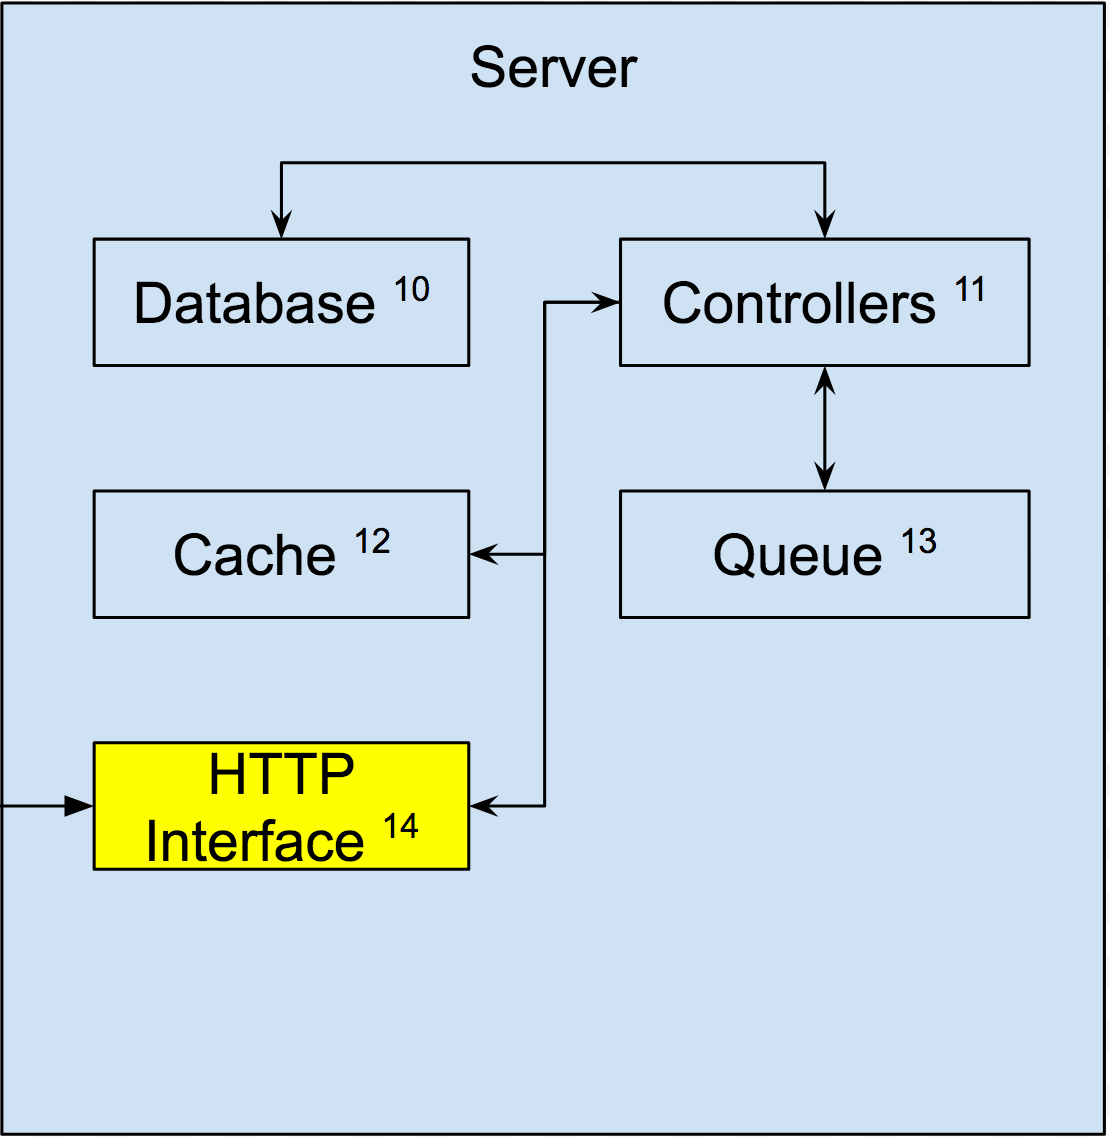
\includegraphics[width=0.60\textwidth]{images/server/server_http_interface.png}
 	\caption{Server-side HTTP Interface subsystem}
\end{figure}

\subsubsection{Assumptions}
N/A

\subsubsection{Responsibilities}
The responsibility of the HTTP interface will include receiving HTTP requests via a chosen open source library, which will request a resource from the controller subsystem. This interface will also make use of Go's built in http package, which will make requests on to the other third party services.

\subsubsection{Subsystem Interfaces}
\begin {table}[H]
\caption {Server-side HTTP Interface interfaces} 
\begin{center}
    \begin{tabular}{ | p{1cm} | p{6cm} | p{3cm} | p{3cm} |}
    \hline
    ID & Description & Inputs & Outputs \\ \hline
    \#01 & Request for login & \pbox{3cm}{JSON containing email and password} & \pbox{3cm}{JSON response containing either users info or an error}  \\ \hline
    \end{tabular}
\end{center}
\end{table}

\newpage

\newpage
\section{Server}
The server is broken down to being a database, controllers for the endpoints, a cache for preserving past results (so that we don't make unnecessary requests each time), a queue to keep track of the requests going out and what order they should be returned in, and finally the interface, that will bring it together with the client.

\begin{figure}[h!]
	\centering
 	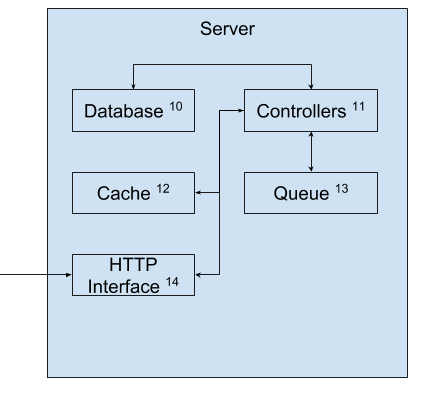
\includegraphics[width=0.60\textwidth]{images/server/ADS-SDS-Server.png}
 	\caption{Server Subsystem}
\end{figure}

\newpage

\subsection{Database}
The database will be used to keep track of user info which includes name, email, passwords, connections (to different services), user preferences, etc.

\begin{figure}[h!]
	\centering
 	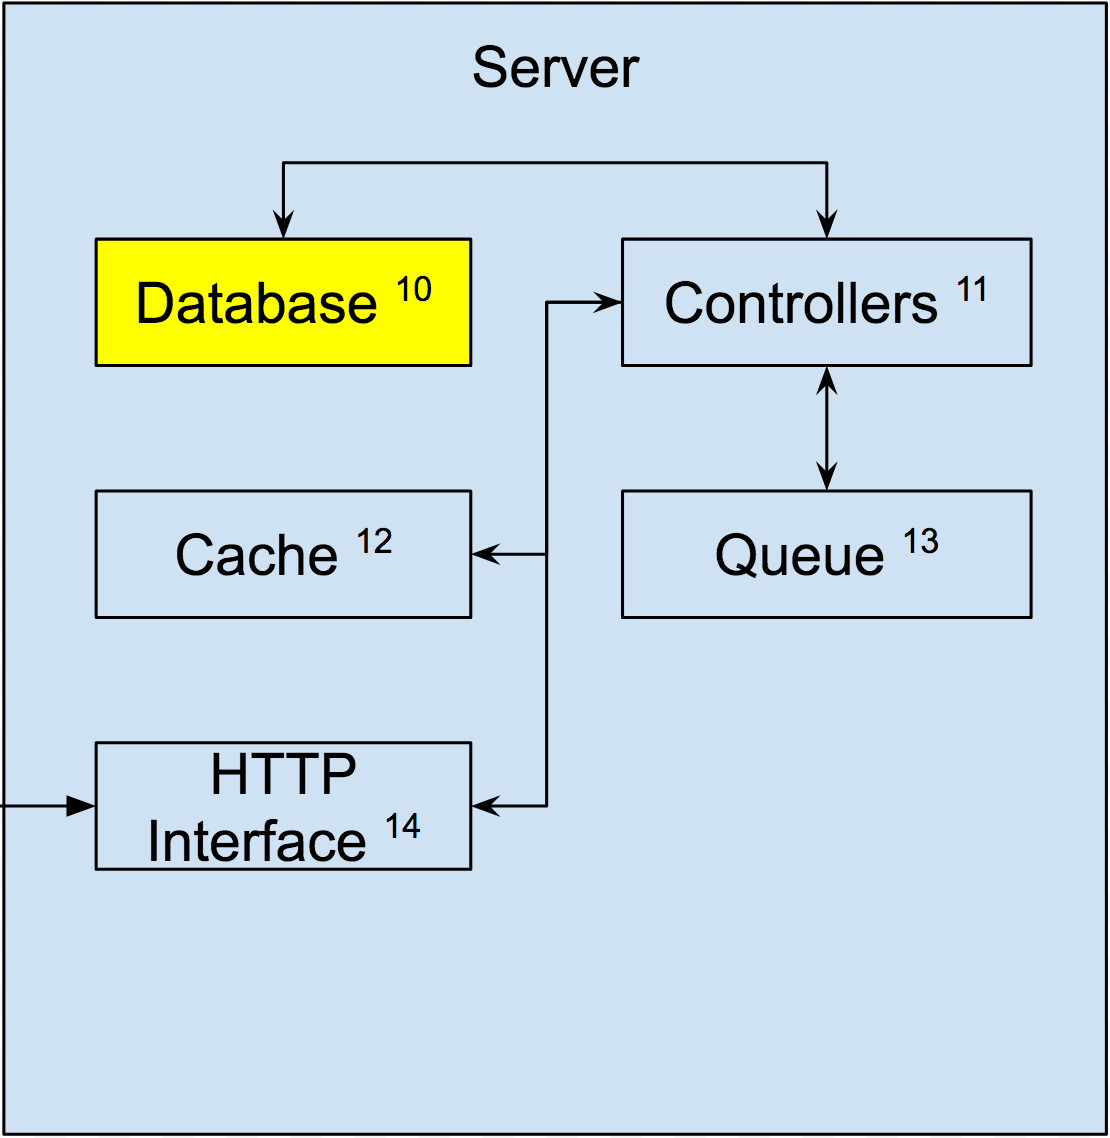
\includegraphics[width=0.60\textwidth]{images/server/server_database.png}
 	\caption{Database subsystem}
\end{figure}

\subsubsection{Assumptions}
N/A

\subsubsection{Responsibilities}
The responsibilities of the database will be to manage user data

\subsubsection{Subsystem Interfaces}
\begin {table}[H]
\caption {Database interfaces} 
\begin{center}
    \begin{tabular}{ | p{1cm} | p{3cm} | p{6cm} | p{6cm} |}
    \hline
    ID & Description & Inputs & Outputs \\ \hline
    \#01 & Store new user & \pbox{6cm}{New user data} & \pbox{6cm}{Confirmation query with new user data saved}  \\ \hline
    \#02 & Returning user login credentials & \pbox{6cm}{Return user e-mail/password} & \pbox{6cm}{Confirmation query with existing user data returned}  \\ \hline
    \end{tabular}
\end{center}
\end{table}

\newpage

\subsection{Controller}

\begin{figure}[h!]
	\centering
 	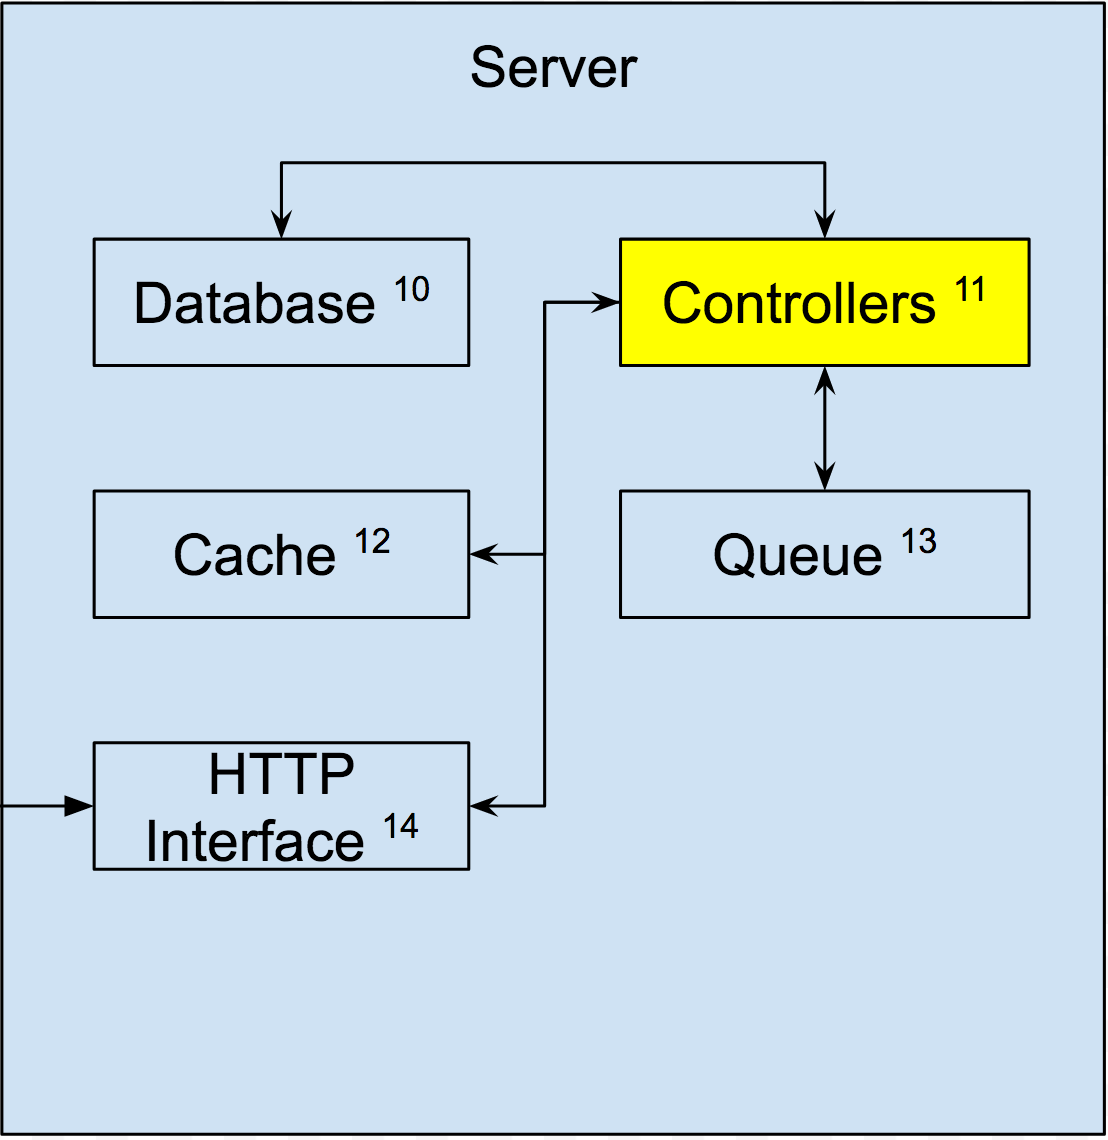
\includegraphics[width=0.60\textwidth]{detailed-design-specification-latex/images/server/server_controller.png}
 \caption{}
\end{figure}

\newpage

\subsubsection{Subsystem Operating System}
This project is primarily software, but we will be hosting our live site using Heroku, so whatever OS they are using for their servers (usually UNIX systems such as macOS, Linux) is our OS. \\

\subsubsection{Subsystem Software Dependencies}
Libraries \\
- Gorilla Mux \\

\subsubsection{Subsystem Programming Languages}
The programming language to be used will be Go. Go is a modern and great programming language to work with and will satisfy our needs to provide an implementation of controller methods.

\subsubsection{Subsystem Data Structures}
The primary data structures that will be returned from the controller will be hash maps and arrays. Internally, the controller will use structs (similar to objects in Object Oriented Programming languages) and arrays.

\subsubsection{Subsystem Data Processing}
To maintain authentication, we use a strategy where we read in each requests header to verify that the user has valid and non-expired token. A token in this context will either allow the user to access the requested resources or direct them to re-authorize. Afterwards, we validate the user has sent in a valid JSON object, and convert it to a map in Go.

\newpage

\subsection{Cache}
The cache will be utilized so that we do not have to make unnecessary requests to the connections when we are grabbing a user content on the respective service

\begin{figure}[h!]
	\centering
 	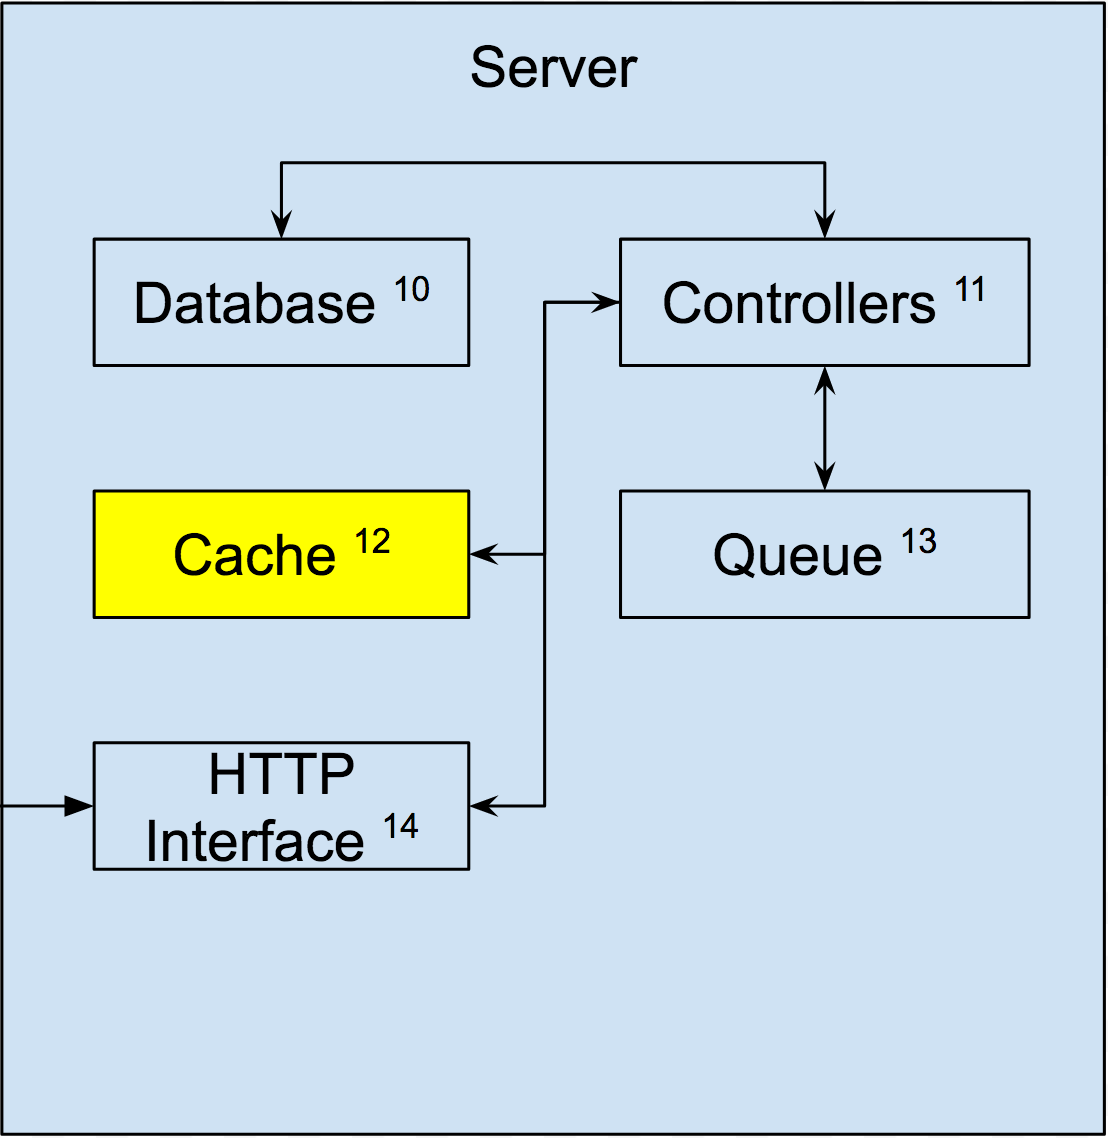
\includegraphics[width=0.60\textwidth]{images/server/server_cache.png}
 	\caption{Cache subsystem}
\end{figure}

\subsubsection{Assumptions}
N/A

\subsubsection{Responsibilities}
To save previous results

\subsubsection{Subsystem Interfaces}
\begin {table}[H]
\caption {Cache interfaces} 
\begin{center}
    \begin{tabular}{ | p{1cm} | p{6cm} | p{6cm} | p{6cm} |}
    \hline
    ID & Description & Inputs & Outputs \\ \hline
    \#01 & Make request & \pbox{3cm}{Retrieve song info} & \pbox{3cm}{Store song info in cache}  \\ \hline
    \end{tabular}
\end{center}
\end{table}

\newpage

\subsection{Queue}
The queue will handle keeping track of requests made and their responses in the order that they are made.

\begin{figure}[h!]
	\centering
 	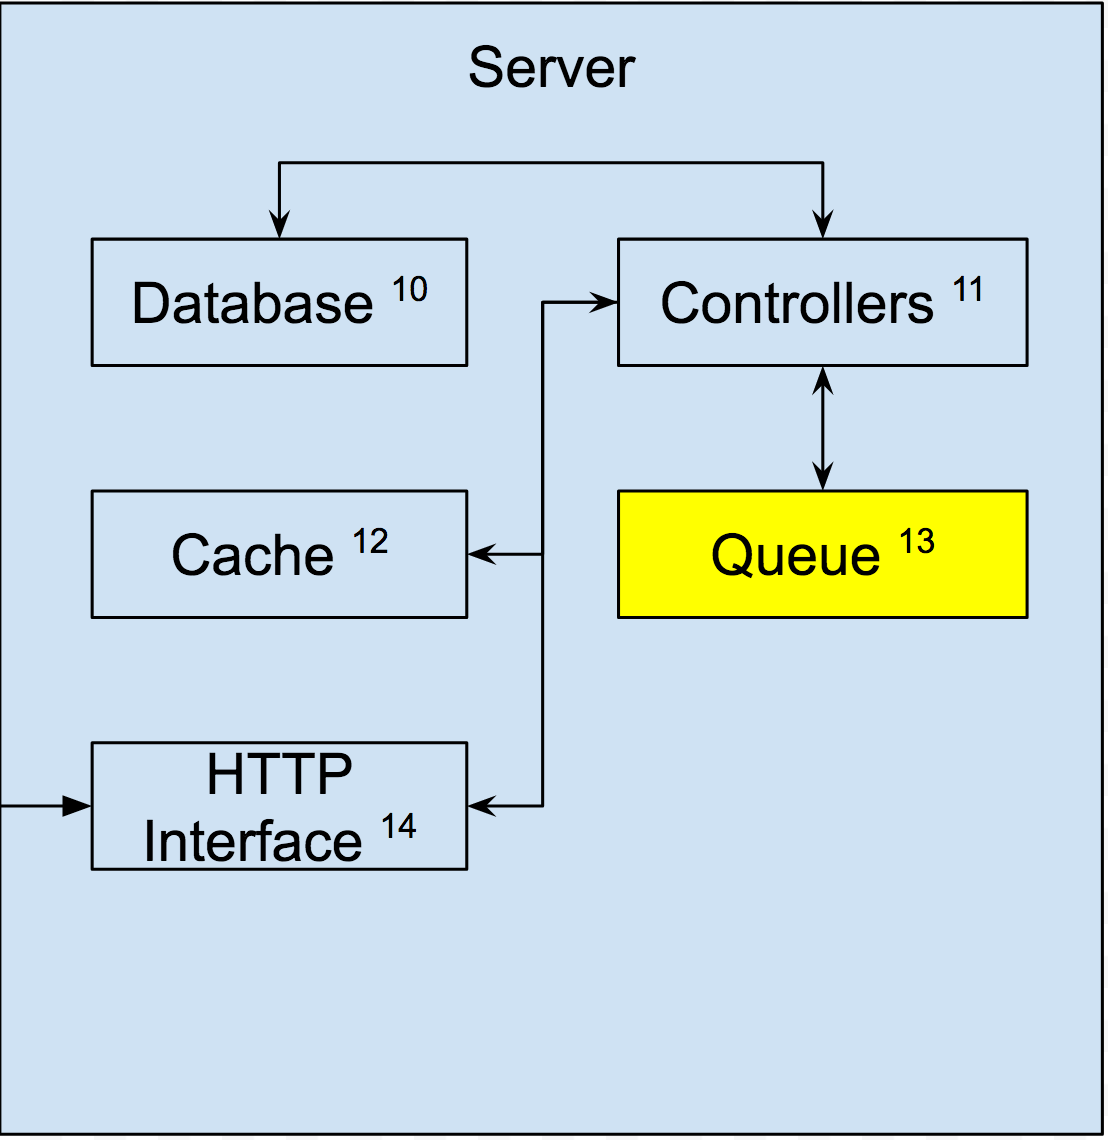
\includegraphics[width=0.60\textwidth]{images/server/server_queue.png}
 	\caption{Queue subsystem}
\end{figure}

\newpage

\subsubsection{Subsystem Hardware}
This project is primarily software, but we will be hosting our live site using Heroku, so whatever hardware they are using for their servers is our hardware.

\\
\subsubsection{Subsystem Operating System}
This project is primarily software, but we will be hosting our live site using Heroku, so whatever OS they are using for their servers (usually UNIX systems such as macOS, Linux) is our OS.

\\
\subsubsection{Subsystem Software Dependencies}
The queue will be implemented as a normal queue (First In First Out) in our chosen programming language, and as such, will not have any dependencies.

\\
\subsubsection{Subsystem Programming Languages}
The programming language to be used will be Go. Go is a modern and great programming language to work with and will satisfy our needs to provide an implementation of a request queue.

\\
\subsubsection{Subsystem Data Structures}
We will be utilizing a regular queue for our request queuing. The data structure used for the queuing will be arrays, and each request that comes through will be appended to our arrays. Then we will be popping the arrays from the front when we are ready to handle the next request.

\\
\subsubsection{Subsystem Data Processing}
The data will be processed in the same way a queue processes data: "First In First Out".

\newpage
\subsection{HTTP Interface}
This interface will be the library used for the server that will direct the incoming request to the controllers via a HTTP/TCP socket.

\begin{figure}[h!]
	\centering
 	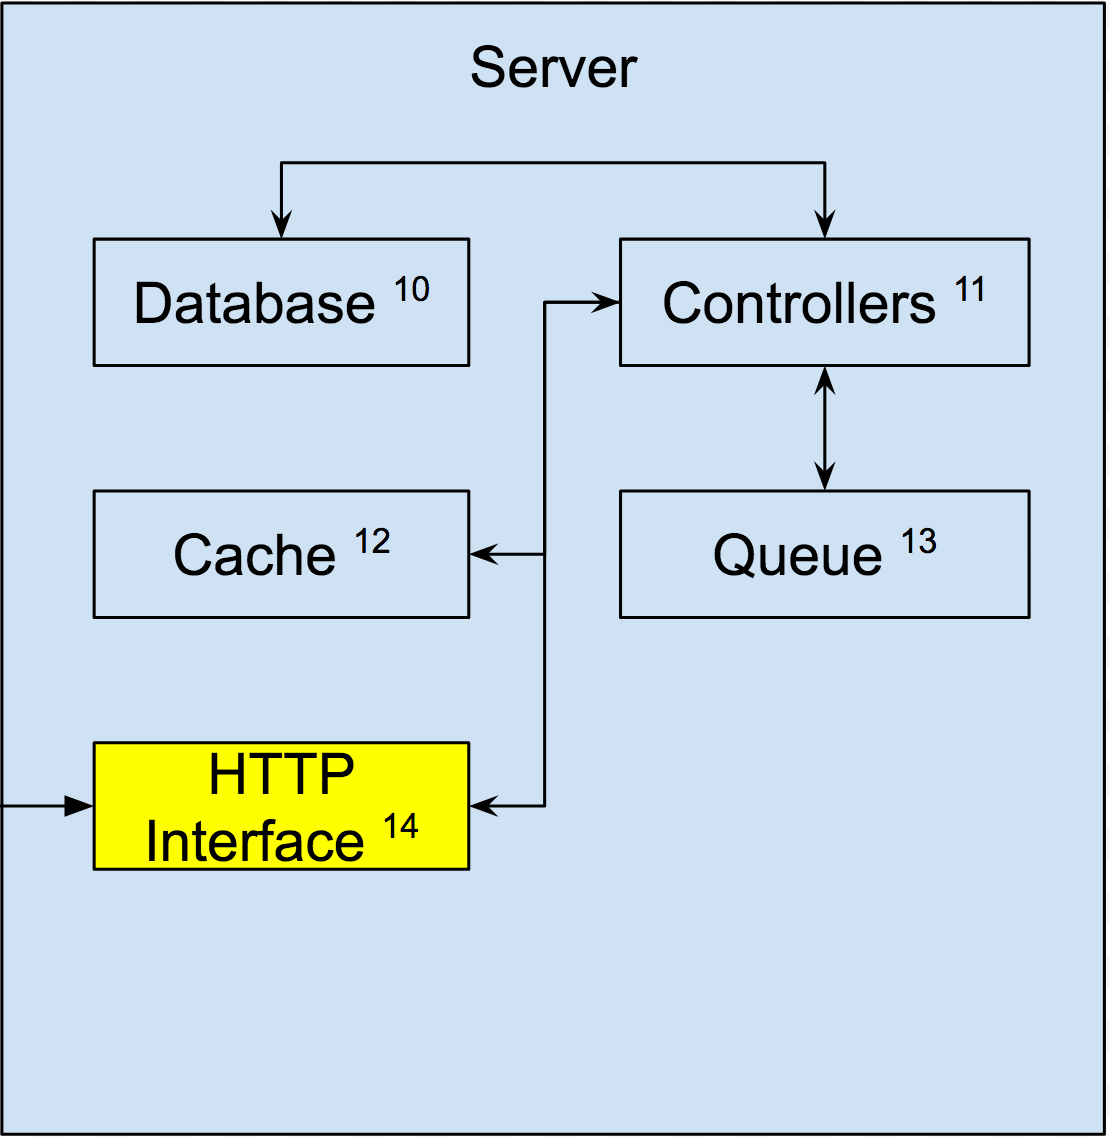
\includegraphics[width=0.60\textwidth]{images/server/server_http_interface.png}
 	\caption{Server-side HTTP Interface subsystem}
\end{figure}

\subsubsection{Assumptions}
N/A

\subsubsection{Responsibilities}
The responsibility of the HTTP interface will include receiving HTTP requests via a chosen open source library, which will request a resource from the controller subsystem. This interface will also make use of Go's built in http package, which will make requests on to the other third party services.

\subsubsection{Subsystem Interfaces}
\begin {table}[H]
\caption {Server-side HTTP Interface interfaces} 
\begin{center}
    \begin{tabular}{ | p{1cm} | p{6cm} | p{3cm} | p{3cm} |}
    \hline
    ID & Description & Inputs & Outputs \\ \hline
    \#01 & Request for login & \pbox{3cm}{JSON containing email and password} & \pbox{3cm}{JSON response containing either users info or an error}  \\ \hline
    \end{tabular}
\end{center}
\end{table}

\newpage

\newpage

%%% References
\bibliographystyle{plain}
\bibliographystyle{reference/IEEEtran_custom}
\bibliography{reference/refs}{}

\end{document}
